%02/10 - Luis del Peso
\chapter{Alineamiento de secuencias por pares}
El alineamiento de secuencias es la herramienta más fundamental de la bioinformática. Permite identificar secuencias relacionadas con una secuencia dada. Como veremos, el parentesco suele implicar que las secuencias pueden tener funciones comunes y esa es una de las principales aplicaciones del alineamiento de secuencias, inferir la función de una secuencia biológica.

\section{Alineamiento de secuencias}
La alineación de secuencias es el procedimiento de ordenar dos (alineación por pares) o varias (alineación de secuencias múltiples, MSA) secuencias intentando colocar el mayor número posible de residuos idénticos o similares en el mismo registro vertical (misma columna). Los residuos no idénticos pueden colocarse en la misma columna como una falta de coincidencia o frente a un hueco en la otra secuencia. El objetivo de la alineación es maximizar el número de coincidencias (residuos idénticos o similares en la misma columna) y minimizar el número de desajustes y huecos.

\begin{figure}[htbp]
\centering
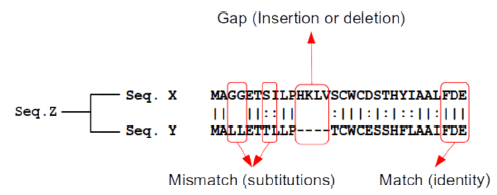
\includegraphics[width = 0.7\textwidth]{figs/pairwise-alignment.png}
\caption{\textbf{Alineamiento por pares.} La alineación por pares modela la evolución de las dos secuencias a partir de un ancestro común. En un intento de colocar los residuos derivados de la misma posición ancestral en el registro vertical, el proceso de alienación maximiza las coincidencias y minimiza las diferencias debidas a mutación de la secuencia ancestral (desajustes y lagunas). En la representación, dos residuos iguales se muestran conectados por una línea vertical. En caso de discordancia, si a nivel biológico los residuos tienen una función similar, se denota con dos puntos, mientras que si la función es diferente, se deja en blanco, al igual que en el caso de inserciones y deleciones.}
\end{figure}

¿Por qué alineamos las secuencias de este modo? En la alineación de secuencias, el supuesto subyacente es que las \textbf{secuencias que se alinean proceden de un ancestro común}. Sin embargo, como consecuencia de las mutaciones acumuladas durante la evolución, las secuencias no serán idénticas. Así pues, el reto consiste en colocar los residuos que derivan de la \textbf{misma posición ancestral} en la misma columna del alineamiento. Sin embargo, sin información sobre la secuencia ancestral y su evolución, lo mejor que podemos hacer es maximizar el número de coincidencias y minimizar el número de discordancias. En las secuencias de proteínas, las sustituciones se producen cuando una mutación (mutación sin sentido o missense) en la secuencia ancestral hace que el codón de un aminoácido se cambie por el de otro. El resultado sería la alineación de dos aminoácidos no idénticos, es decir, un desajuste. Las inserciones y deleciones (normalmente abreviadas como INDEL) se producen cuando se añaden o eliminan residuos de la secuencia ancestral. Las inserciones o deleciones (incluso las de un solo carácter) se representan como huecos en el alineamiento. El número de mutaciones aumentará a medida que las dos secuencias diverjan de su ancestro común. Así, en general, el número de coincidencias disminuye con la distancia evolutiva. En general, se puede inferir que los residuos idénticos entre secuencias probablemente también estén presentes en el ancestro. En el caso de las sustituciones y deleciones/inserciones, no se puede determinar si el ancestro era de una forma u otra, es decir, si realmente se trata de un fragmento que se ha perdido (una deleción) o un fragmento que en algún momento se insertó. 

\section{Comparación de alineamientos}
A la hora de alinear dos secuencias, se pueden producir todos los alineamientos posibles y escoger aquel que tenga el mayor número de coincidencias y el menor número de discordancias o gaps. Un alineamiento óptimo sería aquel que incluya en la misma columna residuos que derivan del mismo residuo original (es decir, alinear residuos ortólogos). Normalmente, no se conoce la secuencia del ancestro o la historia evolutiva, por lo que se intenta inferir al alinear todos los residuos idénticos o similares posibles. Para establecer el grado de similitud, se puede tener en cuenta las propiedades fisicoquímicas (hidrofobicidad, carga neta a pH fisiológico, flexibilidad de la cadena lateral) y la estructura (tamaño, presencia de anillos aromáticos). Además, si se permiten los gaps en el alineamiento, la cantidad de posibles alineamientos aumenta de forma astronómica. Por tanto, para encontrar el mejor alineamiento, se necesita:
\begin{itemize}
\item Una métrica cuantitativa que representa la similitud entre residuos.
\item Un método de puntuación que produce un valor que resume lo buena que es la alineación teniendo en cuenta todas las posiciones y huecos.
\item Un procedimiento capaz de producir todos los alineamientos posibles y puntuarlos eficazmente (y no evaluando todos los posibles alineamientos).
\end{itemize}

\subsection{Matrices de sustitución}
Como ya se ha dicho, el alineamiento consiste en reunir residuos idénticos o similares. Identificar los residuos idénticos es sencillo. Sin embargo, ¿qué entendemos por residuos similares? En el caso de los ácidos nucleicos, la función de un determinado nucleótido (su patrón de emparejamiento de bases) no suele poder sustituirse por ninguno de los demás nucleótidos. Por lo tanto, durante la alineación de secuencias de nucleótidos (normalmente) sólo nos preocupamos por las identidades \footnote{De hecho, dado que las transiciones (es decir, las sustituciones entre las purinas A y G o entre las pirimidinas C y T) son más frecuentes que las transversiones (sustituciones entre purina y pirimidina o viceversa), existen algunos esquemas de puntuación específicos para la alineación de residuos de nucleótidos no idénticos.}. Cualquier otro emparejamiento es un desajuste igualmente perjudicial. Sin embargo, en el caso de las secuencias de aminoácidos, ciertas sustituciones de aminoácidos tienen poco impacto, mientras que otras pueden abolir por completo la función/estructura de la proteína. Así, en el curso de la evolución, los residuos importantes para la función de la molécula tienden a permanecer inalterados o a ser sustituidos por un residuo similar, manteniendo así la estructura y/o la función. Por estas razones, algunas sustituciones particulares se encuentran comúnmente en proteínas relacionadas de diferentes especies. Así, para los alineamientos de proteínas asignamos una puntuación a cada par o aminoácidos que representa la probabilidad de observar la sustitución de uno por otro. Una tabla que contiene las puntuaciones de todos los posibles pares de residuos se denomina \textbf{matriz de sustitución}. Las puntuaciones de cada celda de una matriz de sustitución reflejan la probabilidad de que los dos residuos estén alineados porque son verdaderos homólogos en comparación con la probabilidad de que estén alineados en la misma posición por azar:

$$\frac{p(alineado|homólogo)}{p(alineado|aleatorio)}$$

Estas probabilidades pueden derivarse de \textbf{principios teóricos}, por ejemplo el número de mutaciones necesarias para convertir el codón de un aminoácido en el de otro o la similitud fisicoquímica entre los dos residuos comparados. Sin embargo, las puntuaciones de las matrices de sustitución más populares se han derivado de la \textbf{observación empírica} de las tasas de sustitución en alineaciones de proteínas homólogas. Dos matrices de sustitución populares derivadas empíricamente son PAM y BLOSUM.

\subsubsection{Matrices de sustitución PAM}
Para construir una matriz de sustitución a partir de la observación de los reemplazos ocurridos durante la evolución, sólo necesitamos alinear las proteínas y contar el número de cambios de cada tipo. Sin embargo, generar una matriz de sustituciones a partir de alineamientos de proteínas es un problema circular: se necesita el alineamiento para contar el número de sustituciones observadas pero, para generar un buen alineamiento, se necesitan las puntuaciones de cada par de residuos. Para sortear este problema, Margaret Dayhoff (la primera bioinformática en la historia) y su equipo idearon una estrategia inteligente. Utilizaron secuencias muy similares de homólogos bien conocidos para poder generar alineaciones fácilmente y con gran confianza incluso en ausencia de matrices de sustitución. A continuación, a partir de estos alineamientos generaron árboles filogenéticos que les permitieron inferir la secuencia ancestral de cada par de proteínas alineadas. Por último, a partir de estos árboles calcularon las probabilidades de que cualquier aminoácido mutara en cualquier otro. Así, Dayhoff y sus colegas construyeron árboles filogenéticos a partir de familias de proteínas estrechamente relacionadas y calcularon la probabilidad de que dos residuos alineados derivaran del mismo residuo ancestral (véase la figura \ref{fig:pam}). En este proceso definieron una \textbf{mutación puntual aceptada} (abreviada como PAM) como la sustitución de un residuo original por otro que ha sido aceptado por la selección natural (de lo contrario no estaríamos observando estas secuencias). Como ya se ha mencionado, el conjunto original de proteínas que utilizaron para derivar la matriz de sustitución era muy similar y tenía 1 mutación puntual aceptada por cada 100 residuos de aminoácidos. En consecuencia, esta matriz se denomina PAM1.

Sin embargo, por definición, esta matriz es óptima para puntuar secuencias estrechamente relacionadas, pero no secuencias distantes (está sesgada a secuencias muy próximas evolutivamente). Para generar matrices que reflejaran relaciones más distantes, Dayhoff y sus colegas extrapolaron sus datos observados multiplicando PAM1 por sí mismo varias veces. Cuanto mayor era el número de veces que se multiplicaba el PAM1 por sí mismo, mayor era la distancia que representaba. Por ejemplo, PAM250, derivado de multiplicar PAM1 por sí mismo 250 veces, se utiliza habitualmente para comparar proteínas distantemente relacionadas.

\begin{figure}[htbp]
\centering
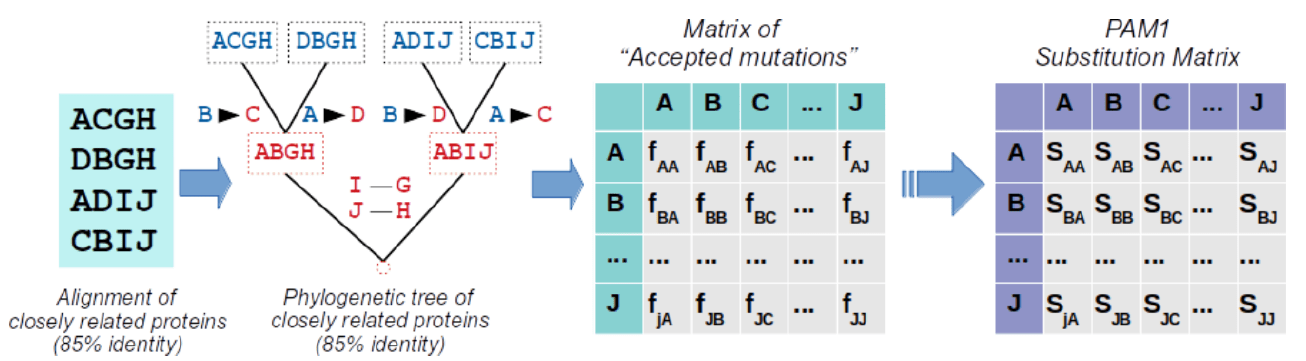
\includegraphics[width = \textwidth]{figs/pam-matrix.png}
\caption{\textbf{Generación de la matriz de sustitución PAM1.} A partir de alineaciones de secuencias estrechamente relacionadas (> 85\% de identidad), Margaret Dayhoff y sus colegas derivaron el árbol filogénico que representaba la evolución de la familia que requería el menor número de mutaciones. A partir de estos árboles contaron el número de veces que cada residuo fue sustituido por cualquier otro y registraron los valores en la matriz de mutaciones aceptadas. Por último, a partir de los datos de esta matriz generaron la matriz de sustitución PAM1 que representa la relación entre la probabilidad de la sustitución observada en el modelo evolutivo (suponiendo homología) y la probabilidad en el modelo aleatorio.}
\label{fig:pam}
\end{figure}

%04/10 - Luis del Peso
\subsubsection{Matrices de sustitución BLOSUM}
Más recientemente, el matrimonio Henikoff utilizó una familia de proteínas más alejada para poder inferir la frecuencia de sustitución en una matriz BLOSUM.

Para evitar la incertidumbre en los alineamientos, Dayhoff utilizó un conjunto de secuencias extremadamente relacionadas para derivar la PAM1. Sin embargo, las matrices PAM para proteínas más distantes se extrapolaron a partir de PAM1 en lugar de derivarse de la observación directa de los alineamientos reales. La acumulación de secuencias de proteínas en bases de datos a lo largo de los años permitió a Henikoff y Henikoff desarrollar un nuevo conjunto de matrices de sustitución a principios de los 90. Estas matrices, denominadas BLOCKS \footnote{un BLOCK se define como una región no superpuesta en el alineamiento de secuencias múltiples de menos de sesenta residuos de aminoácidos} amino acid SUbstitution Matrices (BLOSUM), se generaron al registrar cada posible sustitución de aminoácidos observada en los alineamientos de bloques. Utilizando alineamientos de proteínas que mostraban diferentes porcentajes de identidad, derivaron matrices BLOSUM que representaban la tasa de sustitución observada para diferentes grados de divergencia (figura \ref{fig:blosum}). Para ello, eliminan del bloque todas las secuencias que son idénticas en más de un x\% de posiciones, dejando una única secuencia representativa (por ejemplo, en BLOSUM62 se eliminaron las secuencias que compartían un 62\% de identidad o más). 

\begin{figure}[htbp]
\centering
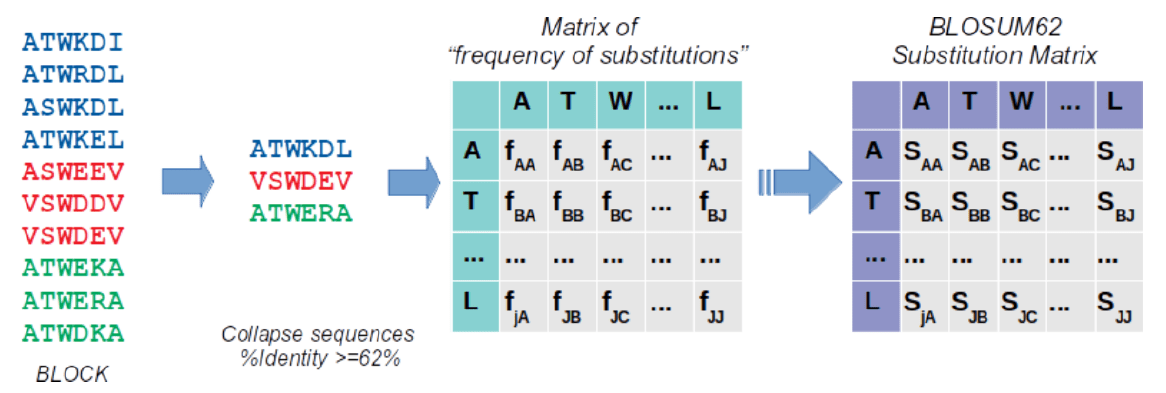
\includegraphics[width = \textwidth]{figs/blosum-matrix.png}
\caption{\textbf{Generación de la matriz de sustitución BLOSUM.} Partiendo de alineaciones sin colapsar de familias de proteínas (BLOCKS), Henikoff y Henikoff derivaron alineaciones que representaban diferentes distancias evolutivas colapsando todas las secuencias del bloque que compartían un umbral, C, de identidad. En la figura C = 62\%, todas las secuencias que comparten un porcentaje de identidad igual o superior al 62\% se muestran en el mismo color de fuente (primera columna), y luego se colapsan en un consenso que representa el clúster (segunda columna). A partir de estos alineamientos, contaron el número de veces que cada residuo i fue sustituido por cualquier otro y registraron los valores en la matriz de frecuencia de sustituciones. Por último, a partir de los datos de esta matriz generaron la matriz de sustituciones BLOSUM62 que representa la relación entre la probabilidad de la sustitución observada en el modelo evolutivo (suponiendo homología) y la probabilidad en el modelo aleatorio.}
\label{fig:blosum}
\end{figure}

Nótese que existen algunas diferencias importantes entre las matrices PAM y BLOSUM. En primer lugar, todas las matrices BLOSUM se derivan de la observación directa de alineamientos, mientras que sólo PAM se deriva de datos y el resto son extrapolaciones. En segundo lugar, mientras que PAM1 se generó a partir de alineaciones de secuencias estrechamente relacionadas (85\% de identidad), las matrices BLOSUM derivan de alineaciones que (pueden) incluir secuencias con un bajo porcentaje de identidad. Por último, para la construcción de PAM se infirieron sustituciones a partir de árboles filogenéticos derivados de los alineamientos. En BLOSUM no se construyó ningún árbol filogenético y las sustituciones se contaron a partir de la observación directa de los residuos alineados. Sin embargo, no se trata de sustituciones reales porque las secuencias alineadas evolucionaron a partir de un ancestro común y entre sí.

\subsubsection{Construcción de matrices de sustitución}
En las secciones anteriores vimos dos estrategias diferentes para determinar la frecuencia de cambios a partir de la observación empírica de alineamientos de proteínas homólogas. Dejando a un lado los detalles, ambos métodos producen una \textbf{matriz de frecuencia de mutación} \footnote{la suma de todas las entradas de la matriz da 1}, donde las entradas $q_{a,b}$, representan la \textbf{probabilidad observada} de encontrar los residuos a y b \textbf{alineados en proteínas homólogas}. En otras palabras, $q_{a,b}$, corresponde al término $p(alineado|homólogo)$. Ahora, para obtener el valor de la entrada para los residuos a y b en la matriz de sustitución correspondiente, necesitamos calcular el término $p(alineado|aleatorio)$, que sería la \textbf{probabilidad esperada}. En el modelo aleatorio suponemos que las dos proteínas alineadas no están relacionadas y no existen restricciones estructurales o funcionales que puedan causar correlación entre los residuos en una posición dada. Así, en este modelo la probabilidad de encontrar los residuos a y b alineados sólo depende de su frecuencia en las proteínas. En el modelo aleatorio no existe correlación alguna entre los residuos alineados en una posición dada, por lo que la probabilidad de observar a en una secuencia y b en la otra son independientes de modo que:

$$p(alineado|aleatorio) = p(a \cap b) = p_a p_b $$

donde $p_a$, y $p_b$, son las frecuencias de a y b respectivamente. La probabilidad de observar a y b alineados en estos dos modelos puede compararse tomando el cociente de las probabilidades, denominado \textbf{odds ratio}: $q_{a,b}/(p_a p_b)$. Cuando la probabilidad en el modelo evolutivo es mayor que en el modelo aleatorio, el odds-ratio toma cualquier valor entre 1 e infinito. Sin embargo, cuando la probabilidad en el modelo aleatorio es mayor, la odds-ratio está entre 0 y 1. Para evitar esta asimetría, se suele tomar el logaritmo de la odds-ratio para obtener la \textbf{log-odds ratio}. Como veremos más adelante, tomar el logaritmo del odds-ratio también facilita el cálculo de la puntuación total de la alineación. Por lo tanto, la entrada en la matriz de sustitución correspondiente a a y b se calcula como:

$$ s_{a, b} = log \frac{q_{a, b}}{p_a p_b} = log \frac{p(cambio|modelo evolutivo)}{p(cambio|aleatorio)} = log \frac{p(observado)}{p(esperado)} $$

La figura \ref{fig:substitution} muestra las matrices de sustitución PAM250 y BLOSUM62. Dado que la puntuación del alineamiento a sobre b es la misma de b sobre a, estas matrices son simétricas. Por este motivo, normalmente sólo se representa la mitad de la matriz. Los números positivos significan que se han observado más veces el cambio de residuos que lo que cabría esperar por azar, por lo que debe haber alguna presión positiva para que se mantenga. En el caso de los números negativos, se debe a una selección negativa. Cuando es 0, el ratio es 1 y por tanto la frecuencia es la observada por azar, no hay ninguna presión. 

Un ejemplo: El triptófano tiene una frecuencia de mutación observada muy pequeña, pero en la tabla BLOSUM, su número es el más alto. Esto significa que es un aminoácido muy importante que no se puede cambiar por ningún otro. Así, la tabla de frecuencias per se no refleja el parecido entre residuos, ya que hay que tener en cuenta la frecuencia. Sin embargo, la tabla BLOSUM sí refleja el parecido entre los residuos.   

\begin{figure}[htbp]
\centering
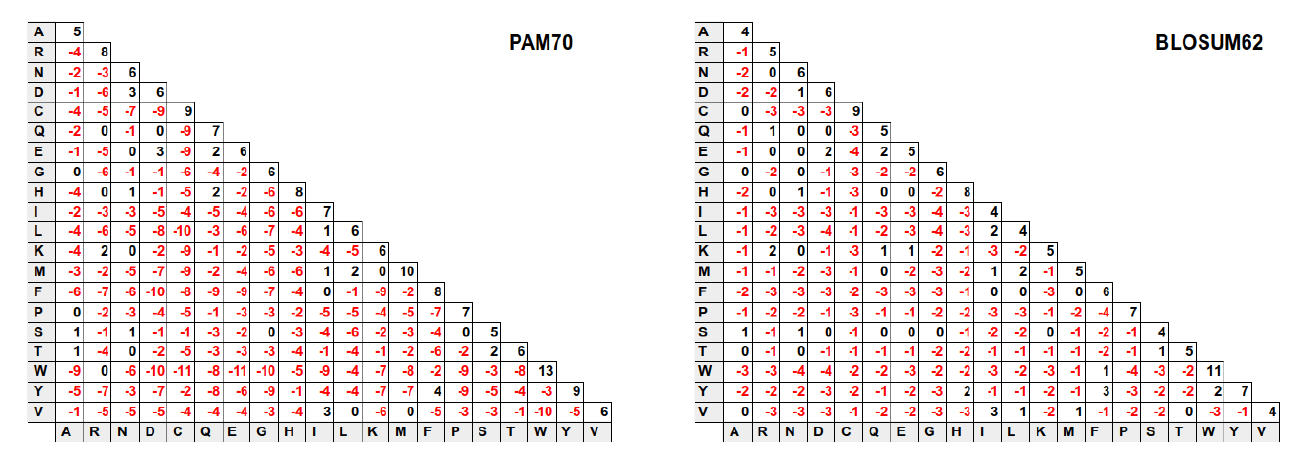
\includegraphics[width = \textwidth]{figs/substitution-matrix.png}
\caption{\textbf{Matrices de sustitución de aminoácidos.} La figura muestra las matrices de sustitución PAM250 (izquierda) y BLOSUM62 (derecha). Los valores negativos (en rojo) indican las sustituciones que tienen más probabilidades de observarse en el modelo aleatorio que en el evolutivo.}
\label{fig:substitution}
\end{figure}

\begin{table}[htbp]
\begin{mdframed}[backgroundcolor=black!10]
\textbf{Ejemplo de cálculo de matriz puntuación y odds ratio: Cambio D-L} \\
La matriz de frecuencia de mutación observada indica que el cambio D-L se ha observado 15 veces en 10000, es decir, 15/10000. La frecuencia de los bloques es 0,054 para D y 0,099 para L. Esto representa la frecuencia esperada. La puntuación se calcularía siguiendo la fórmula:

$$s = 2 \cdot \log_2(odds ratio) = 2 \cdot \log_2(\frac{observado}{esperado})$$

Sustituyendo los valores:

$$s = 2 \cdot \log_2(\frac{15/10000}{0,054 \cdot 0,099}) = -3,66 \approx -4$$

Cuando hay números decimales, se redondea al siguiente número entero. Al comprobar el valor en la matriz BLOSUM, el resultado efectivamente es -4.
\end{mdframed}
\end{table}

\begin{figure}[htbp]
\centering
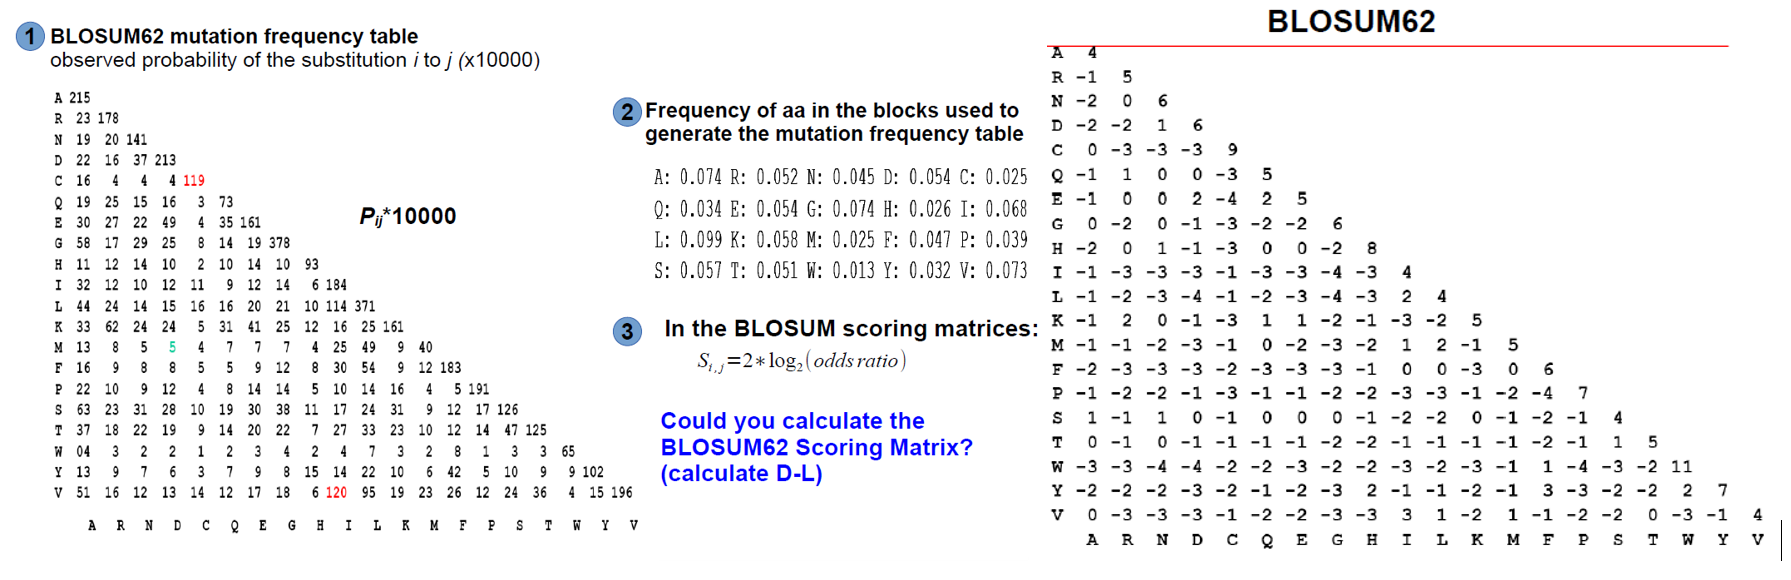
\includegraphics[width = \textwidth]{figs/ejercicio-blosum.png}
\end{figure}

\subsection{Alineamientos de puntuación (scoring alignments)}
Las matrices de sustitución ofrecen un método para puntuar posiciones individuales. Sin embargo, para comparar diferentes alineaciones, necesitamos un único valor que represente la puntuación combinada de todas las posiciones. Para calcular dicha puntuación, suponemos que cada posición del alineamiento es independiente de las demás \footnote{Nótese que esto es probablemente una simplificación excesiva porque en las proteínas reales a menudo existe una correlación entre residuos adyacentes. Por ejemplo, en una hélice anfipática los residuos polares e hidrófobos se distribuyen en caras opuestas. Por lo tanto, habrá cierta correlación entre los residuos en ciertas posiciones.} y calculamos la puntuación del alineamiento S como la suma de las puntuaciones individuales de cada una de las n posiciones, siendo s la entrada de la matriz de sustitución para los residuos a y b en la posición i.

$$S = \sum_{i = 1}^{n} (s_{a,b})_i$$

En otras palabras, se pueden sumar los valores de las matrices BLOSUM de cada posición al haber utilizado el logaritmo. Ahora, esta función de puntuación sólo funciona para coincidencias y discordancias pero no tiene en cuenta los INDELs. Para representar los INDEL, un residuo o una serie de residuos en una secuencia de la alineación se empareja con guiones («-») en la otra secuencia. Durante la puntuación, la presencia de un hueco en el alineamiento da lugar a una penalización por hueco que se resta de la puntuación total. Hay dos razones para penalizar los huecos. En primer lugar, un hueco implica una diferencia entre las secuencias comparadas y, por tanto, reduce nuestra certeza sobre su origen común. Los huecos corresponden a eventos de inserción/deleción que ocurrieron durante la evolución desde el ancestro común en uno de los linajes. Por lo tanto, en general, cuanto mayor sea el número de huecos, mayor será la distancia evolutiva entre las secuencias. La segunda razón es que, introduciendo un número ridículo de huecos, podríamos aumentar artificialmente el número de coincidencias y, como consecuencia, aumentar la puntuación del alineamiento, aunque el alineamiento resultante no tendría sentido desde el punto de vista biológico. Así, las penalizaciones por huecos actúan limitando la introducción de huecos. Por lo general, el usuario establece la penalización por hueco a partir de un conjunto de valores predefinidos \footnote{En algunos programas, la penalización por hueco varía en función del tipo de residuo con el que se alinea el hueco. La razón es que algunos residuos tienden a estar fuertemente conservados debido a su impacto en la estructura/función. Por lo tanto, es más probable que la supresión de esos residuos altere la estructura/función y, por lo tanto, sufra selección negativa.} que se han determinado empíricamente a partir de la observación de su efecto en los alineamientos.

